\documentclass[a4paper, 12pt]{article}

% Paquetes básicos para idioma y codificación
\usepackage[utf8]{inputenc}
\usepackage[T1]{fontenc}
\usepackage[spanish]{babel}

% Paquete para insertar imágenes
\usepackage{graphicx}

% --- PAQUETE NUEVO PARA FORZAR LA POSICIÓN DE LAS IMÁGENES ---
\usepackage{float} 

% Paquete para que el índice tenga enlaces clickeables
\usepackage[colorlinks=true, linkcolor=black, urlcolor=blue]{hyperref}

% Configuración del título
\title{Memoria de Prácticas: Ingeniería de Servidores}
\author{Juan Reche Aguilar}
\date{\today}

\begin{document}

% Genera la portada con el título
\maketitle
\clearpage % Usamos clearpage en lugar de newpage

\section{Ejercicio 5: Ansible}
% Imagen 1
\begin{figure}[H]
    \centering
    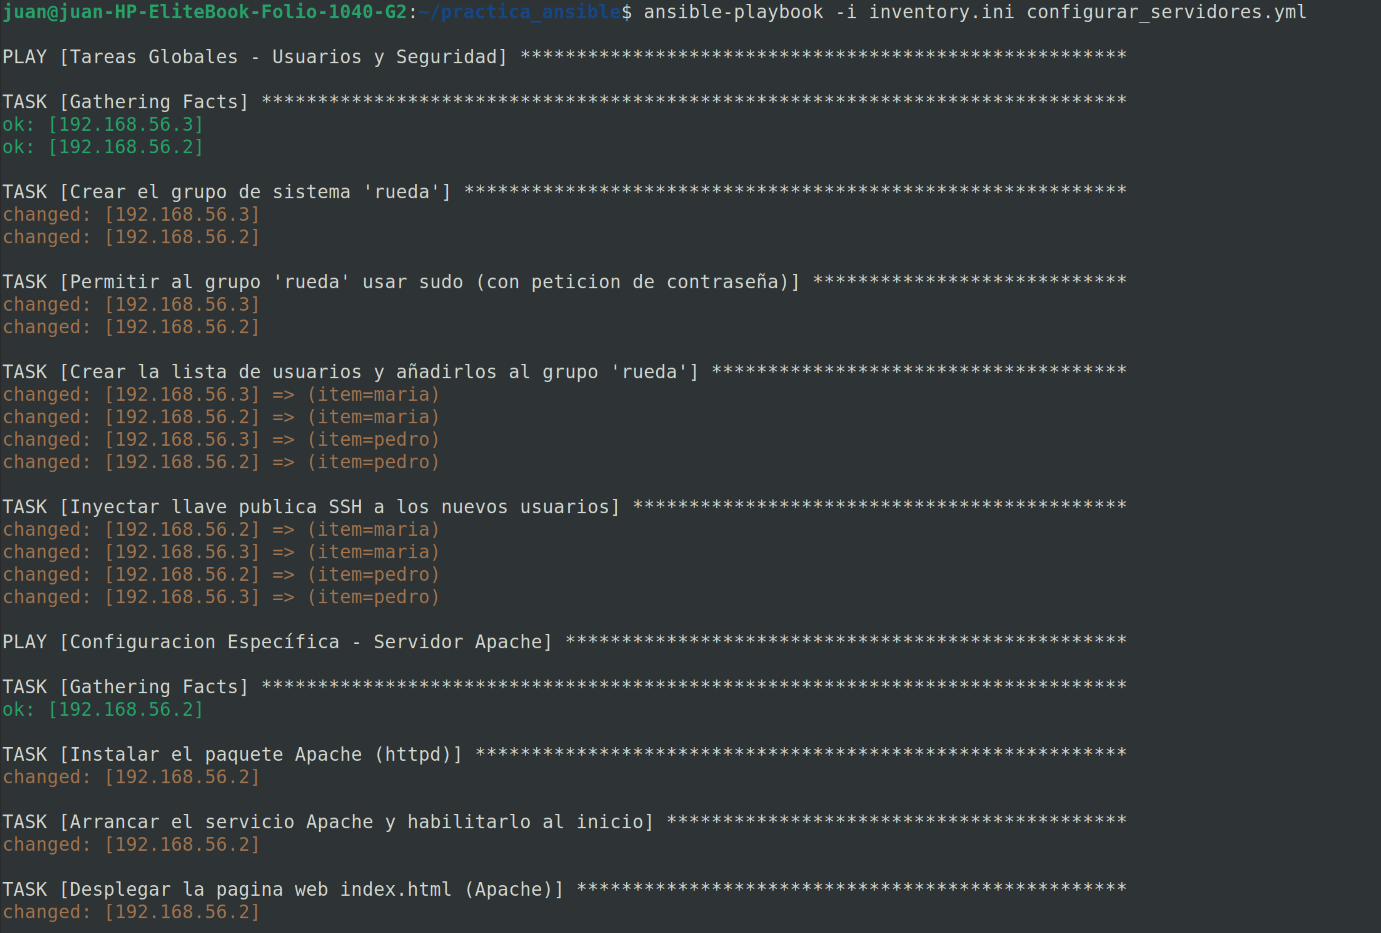
\includegraphics[width=0.8\textwidth]{../ej5/ej5_1.png}
    \caption{Parte 1 de la ejecucion del playbook de Ansible}
\end{figure}

% Imagen 2
\begin{figure}[H]
    \centering
    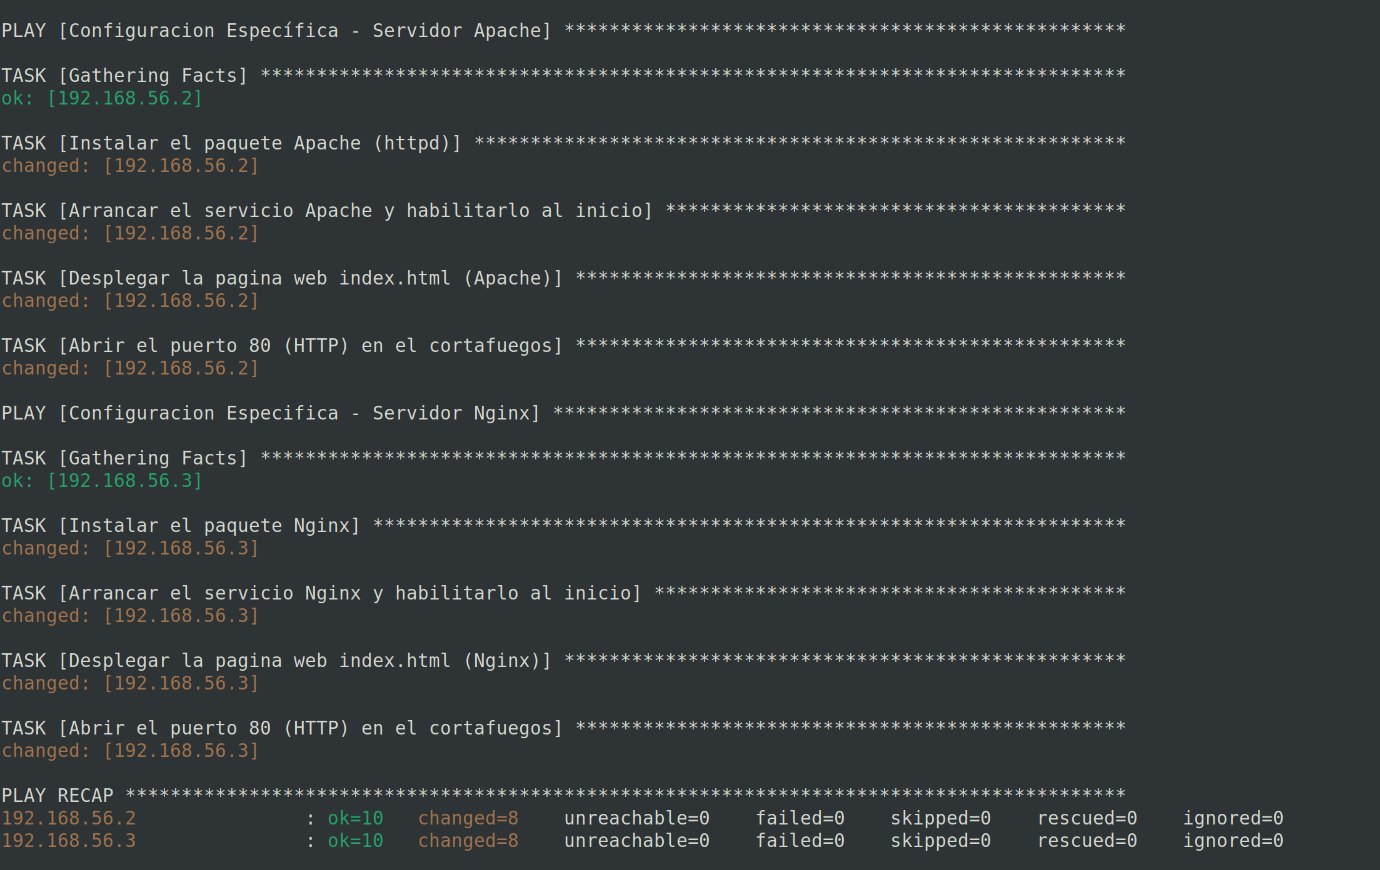
\includegraphics[width=0.8\textwidth]{../ej5/ej5_2.png}
    \caption{Parte 2 de la ejecucion del playbook de Ansible}
\end{figure}

% Imagen 3
\begin{figure}[H]
    \centering
    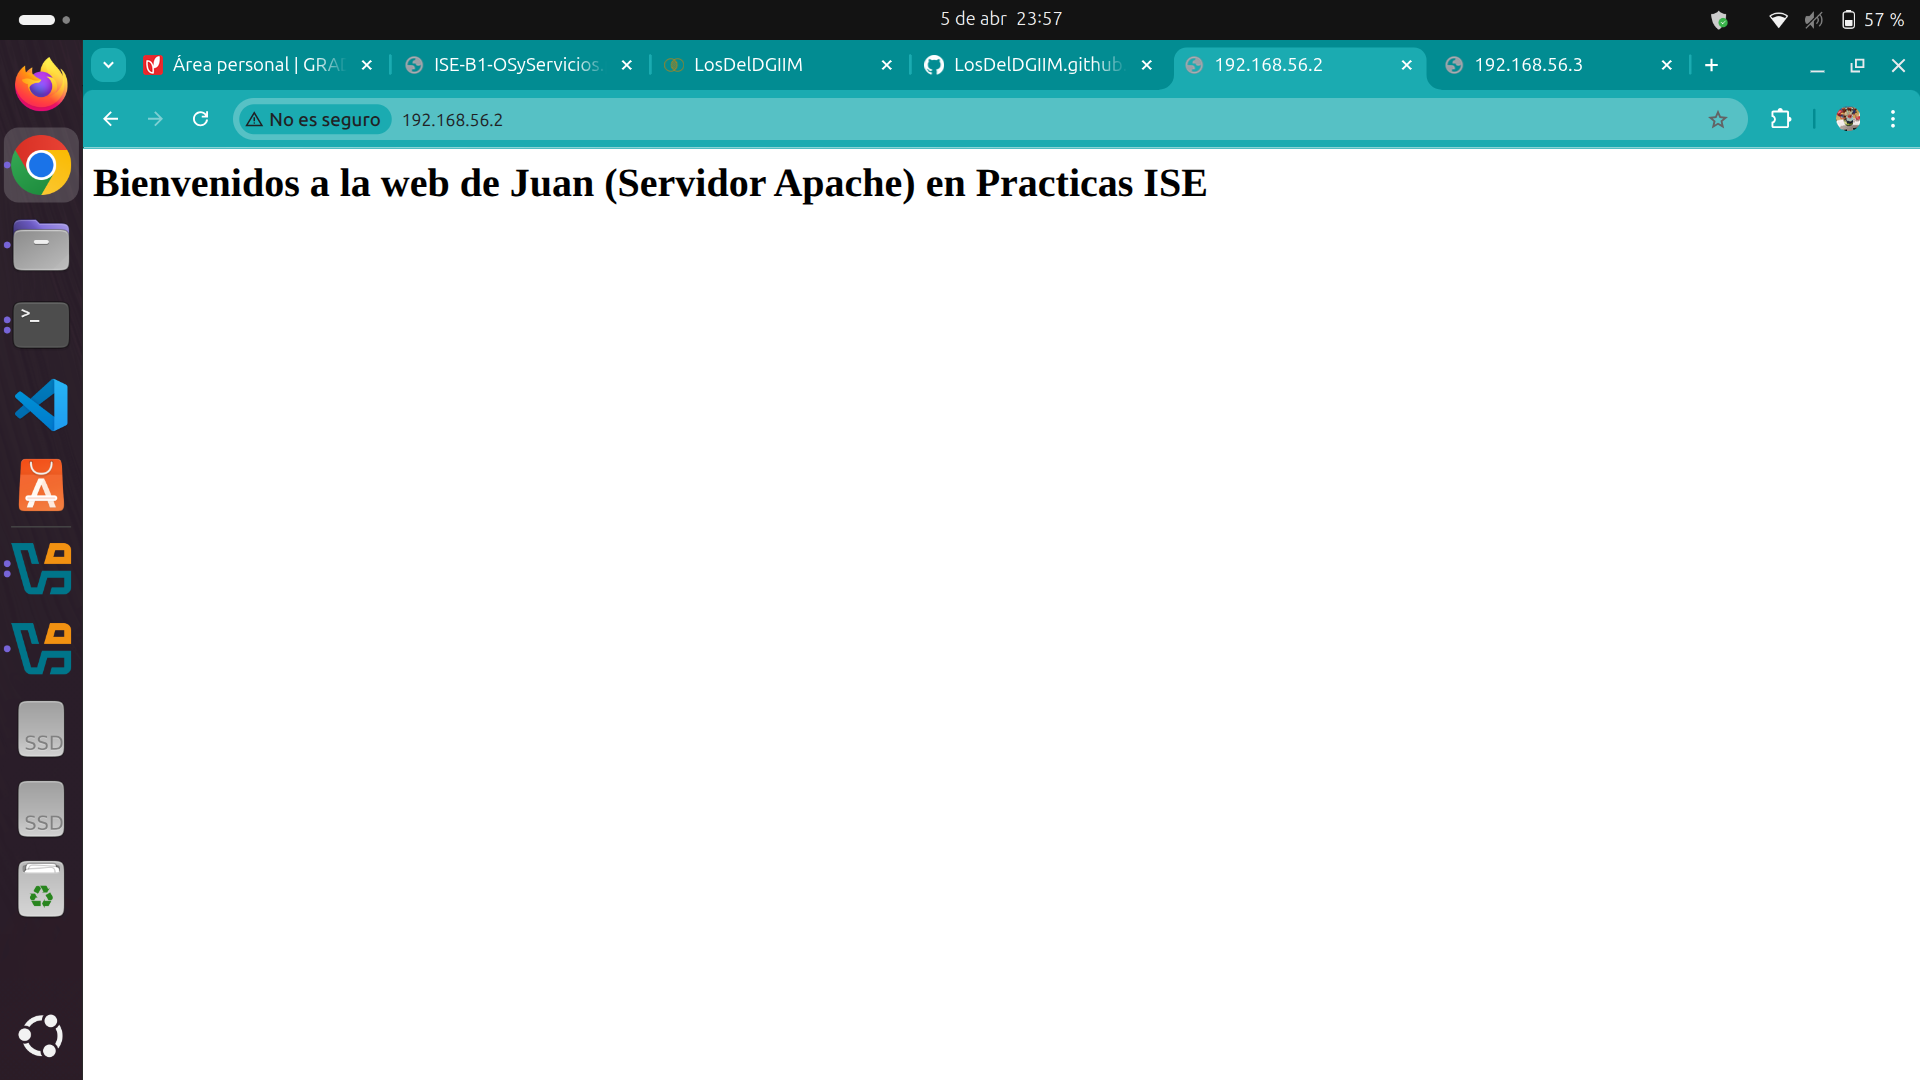
\includegraphics[width=0.8\textwidth]{../ej5/ej5_3.png}
    \caption{Comprobacion de Apache}
\end{figure}

% Imagen 4
\begin{figure}[H]
    \centering
    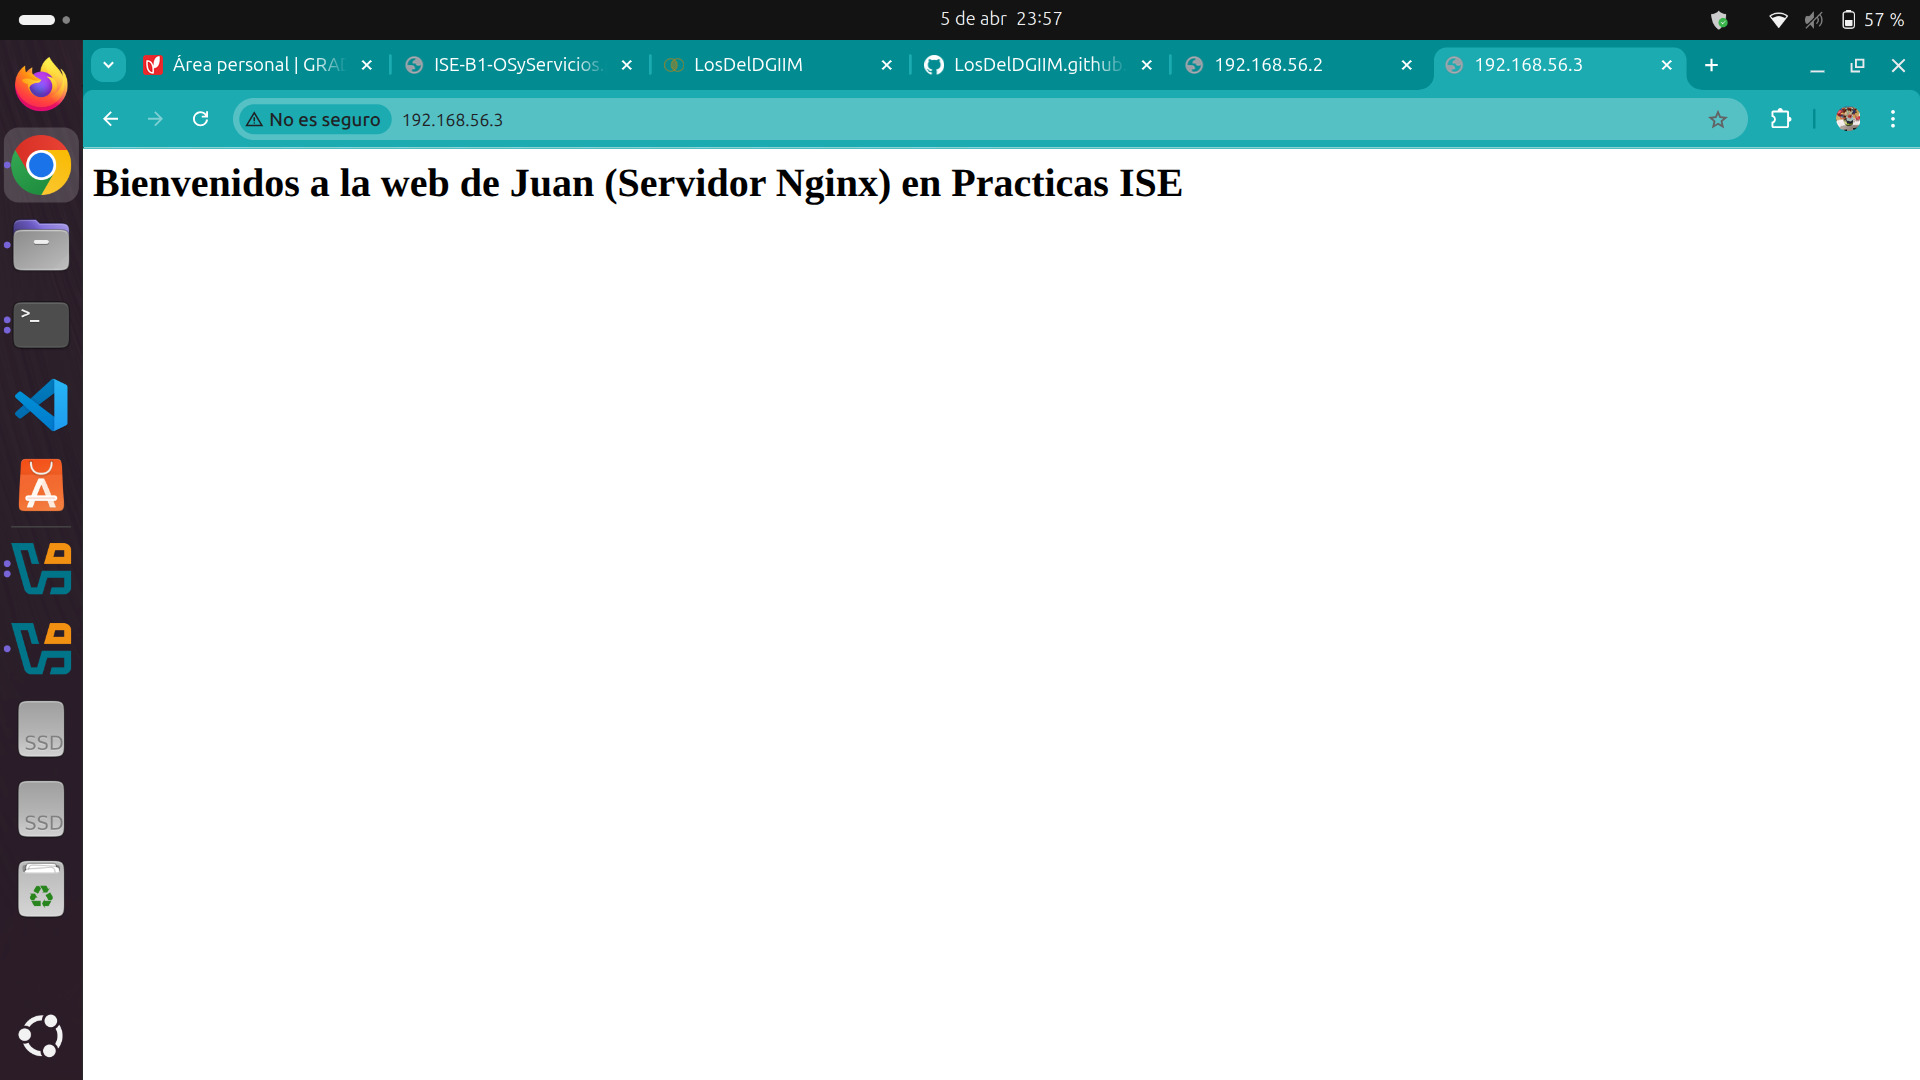
\includegraphics[width=0.8\textwidth]{../ej5/ej5_4.png}
    \caption{Comprobacion de Nginx}
\end{figure}

% Imagen 5
\begin{figure}[H]
    \centering
    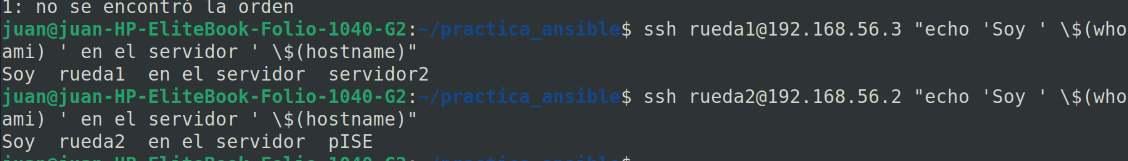
\includegraphics[width=0.8\textwidth]{../ej5/ej5_5.png}
    \caption{Comprobacion mediante ping de la conexion ssh de los usuarios 
    creados por el playbook de Ansible del grupo rueda}
\end{figure}

\end{document}
